\documentclass{standalone}
\usepackage{mathpazo}
\usepackage[american]{circuitikz}

\begin{document}
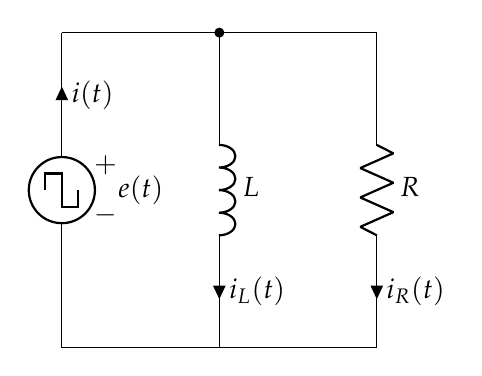
\begin{tikzpicture}
  \coordinate (A) at (0,4);
  \coordinate (B) at (2,4);
  \coordinate (C) at (4,4);
  \coordinate (D) at (0,0);
  \coordinate (E) at (2,0);
  \coordinate (F) at (4,0);
  \draw
  (A) to [short] (C)
  to [R, l = $R$, i= $i_R(t)$] (F)
  to [short] (D);
  \draw
  (A) to [sqV, v=$e(t)$, i<= $i(t)$] (D);
  \draw
  (B) to [L, *-, l=$L$, i = $i_L(t)$] (E);
  \end{tikzpicture}
\end{document}